%\documentclass[slides]{beamer} %switch "slides" to "handout" for printing out
\documentclass[handout]{beamer}

%packages
%\usepackage{latexsym}
\usepackage{graphicx}
\usepackage{color}
\usepackage{amsmath}
\usepackage{dsfont}
\usepackage{placeins}
\usepackage{amssymb}
\usepackage{wasysym}
\usepackage{abstract}
\usepackage{hyperref}
\usepackage{etoolbox}
\usepackage{datetime}
\usepackage{xcolor}
\usepackage{alphalph}
\settimeformat{ampmtime}

%\usepackage{pstricks,pst-node,pst-tree}

%\usepackage{algpseudocode}
%\usepackage{amsthm}
%\usepackage{hyperref}
%\usepackage{mathrsfs}
%\usepackage{amsfonts}
%\usepackage{bbding}
%\usepackage{listings}
%\usepackage{appendix}
\usepackage[margin=1in]{geometry}
%\geometry{papersize={8.5in,11in},total={6.5in,9in}}
%\usepackage{cancel}
%\usepackage{algorithmic, algorithm}

\makeatletter
\def\maxwidth{ %
  \ifdim\Gin@nat@width>\linewidth
    \linewidth
  \else
    \Gin@nat@width
  \fi
}
\makeatother

\definecolor{fgcolor}{rgb}{0.345, 0.345, 0.345}
\newcommand{\hlnum}[1]{\textcolor[rgb]{0.686,0.059,0.569}{#1}}%
\newcommand{\hlstr}[1]{\textcolor[rgb]{0.192,0.494,0.8}{#1}}%
\newcommand{\hlcom}[1]{\textcolor[rgb]{0.678,0.584,0.686}{\textit{#1}}}%
\newcommand{\hlopt}[1]{\textcolor[rgb]{0,0,0}{#1}}%
\newcommand{\hlstd}[1]{\textcolor[rgb]{0.345,0.345,0.345}{#1}}%
\newcommand{\hlkwa}[1]{\textcolor[rgb]{0.161,0.373,0.58}{\textbf{#1}}}%
\newcommand{\hlkwb}[1]{\textcolor[rgb]{0.69,0.353,0.396}{#1}}%
\newcommand{\hlkwc}[1]{\textcolor[rgb]{0.333,0.667,0.333}{#1}}%
\newcommand{\hlkwd}[1]{\textcolor[rgb]{0.737,0.353,0.396}{\textbf{#1}}}%

\usepackage{framed}
\makeatletter
\newenvironment{kframe}{%
 \def\at@end@of@kframe{}%
 \ifinner\ifhmode%
  \def\at@end@of@kframe{\end{minipage}}%
  \begin{minipage}{\columnwidth}%
 \fi\fi%
 \def\FrameCommand##1{\hskip\@totalleftmargin \hskip-\fboxsep
 \colorbox{shadecolor}{##1}\hskip-\fboxsep
     % There is no \\@totalrightmargin, so:
     \hskip-\linewidth \hskip-\@totalleftmargin \hskip\columnwidth}%
 \MakeFramed {\advance\hsize-\width
   \@totalleftmargin\z@ \linewidth\hsize
   \@setminipage}}%
 {\par\unskip\endMakeFramed%
 \at@end@of@kframe}
\makeatother

\definecolor{shadecolor}{rgb}{.77, .77, .77}
\definecolor{messagecolor}{rgb}{0, 0, 0}
\definecolor{warningcolor}{rgb}{1, 0, 1}
\definecolor{errorcolor}{rgb}{1, 0, 0}
\newenvironment{knitrout}{}{} % an empty environment to be redefined in TeX

\usepackage{alltt}
\usepackage[T1]{fontenc}

\newcommand{\qu}[1]{``#1''}
\newcounter{probnum}
\setcounter{probnum}{1}

%create definition to allow local margin changes
\def\changemargin#1#2{\list{}{\rightmargin#2\leftmargin#1}\item[]}
\let\endchangemargin=\endlist 

%allow equations to span multiple pages
\allowdisplaybreaks

%define colors and color typesetting conveniences
\definecolor{gray}{rgb}{0.5,0.5,0.5}
\definecolor{black}{rgb}{0,0,0}
\definecolor{white}{rgb}{1,1,1}
\definecolor{blue}{rgb}{0.5,0.5,1}
\newcommand{\inblue}[1]{\color{blue}#1 \color{black}}
\definecolor{green}{rgb}{0.133,0.545,0.133}
\newcommand{\ingreen}[1]{\color{green}#1 \color{black}}
\definecolor{yellow}{rgb}{1,1,0}
\newcommand{\inyellow}[1]{\color{yellow}#1 \color{black}}
\definecolor{orange}{rgb}{0.9,0.649,0}
\newcommand{\inorange}[1]{\color{orange}#1 \color{black}}
\definecolor{red}{rgb}{1,0.133,0.133}
\newcommand{\inred}[1]{\color{red}#1 \color{black}}
\definecolor{purple}{rgb}{0.58,0,0.827}
\newcommand{\inpurple}[1]{\color{purple}#1 \color{black}}
\definecolor{backgcode}{rgb}{0.97,0.97,0.8}
\definecolor{Brown}{cmyk}{0,0.81,1,0.60}
\definecolor{OliveGreen}{cmyk}{0.64,0,0.95,0.40}
\definecolor{CadetBlue}{cmyk}{0.62,0.57,0.23,0}

%define new math operators
\DeclareMathOperator*{\argmax}{arg\,max~}
\DeclareMathOperator*{\argmin}{arg\,min~}
\DeclareMathOperator*{\argsup}{arg\,sup~}
\DeclareMathOperator*{\arginf}{arg\,inf~}
\DeclareMathOperator*{\convolution}{\text{\Huge{$\ast$}}}
\newcommand{\infconv}[2]{\convolution^\infty_{#1 = 1} #2}
%true functions

%%%% GENERAL SHORTCUTS

%shortcuts for pure typesetting conveniences
\newcommand{\bv}[1]{\boldsymbol{#1}}

%shortcuts for compound constants
\newcommand{\BetaDistrConst}{\dfrac{\Gamma(\alpha + \beta)}{\Gamma(\alpha)\Gamma(\beta)}}
\newcommand{\NormDistrConst}{\dfrac{1}{\sqrt{2\pi\sigma^2}}}

%shortcuts for conventional symbols
\newcommand{\tsq}{\tau^2}
\newcommand{\tsqh}{\hat{\tau}^2}
\newcommand{\sigsq}{\sigma^2}
\newcommand{\sigsqsq}{\parens{\sigma^2}^2}
\newcommand{\sigsqovern}{\dfrac{\sigsq}{n}}
\newcommand{\tausq}{\tau^2}
\newcommand{\tausqalpha}{\tau^2_\alpha}
\newcommand{\tausqbeta}{\tau^2_\beta}
\newcommand{\tausqsigma}{\tau^2_\sigma}
\newcommand{\betasq}{\beta^2}
\newcommand{\sigsqvec}{\bv{\sigma}^2}
\newcommand{\sigsqhat}{\hat{\sigma}^2}
\newcommand{\sigsqhatmlebayes}{\sigsqhat_{\text{Bayes, MLE}}}
\newcommand{\sigsqhatmle}[1]{\sigsqhat_{#1, \text{MLE}}}
\newcommand{\bSigma}{\bv{\Sigma}}
\newcommand{\bSigmainv}{\bSigma^{-1}}
\newcommand{\thetavec}{\bv{\theta}}
\newcommand{\thetahat}{\hat{\theta}}
\newcommand{\thetahatmle}{\hat{\theta}_{\mathrm{MLE}}}
\newcommand{\thetavechatmle}{\hat{\thetavec}_{\mathrm{MLE}}}
\newcommand{\muhat}{\hat{\mu}}
\newcommand{\musq}{\mu^2}
\newcommand{\muvec}{\bv{\mu}}
\newcommand{\muhatmle}{\muhat_{\text{MLE}}}
\newcommand{\lambdahat}{\hat{\lambda}}
\newcommand{\lambdahatmle}{\lambdahat_{\text{MLE}}}
\newcommand{\etavec}{\bv{\eta}}
\newcommand{\alphavec}{\bv{\alpha}}
\newcommand{\minimaxdec}{\delta^*_{\mathrm{mm}}}
\newcommand{\ybar}{\bar{y}}
\newcommand{\xbar}{\bar{x}}
\newcommand{\Xbar}{\bar{X}}
\newcommand{\phat}{\hat{p}}
\newcommand{\Phat}{\hat{P}}
\newcommand{\Zbar}{\bar{Z}}
\newcommand{\iid}{~{\buildrel iid \over \sim}~}
\newcommand{\inddist}{~{\buildrel ind \over \sim}~}
\newcommand{\approxdist}{~{\buildrel approx \over \sim}~}
\newcommand{\equalsindist}{~{\buildrel d \over =}~}
\newcommand{\loglik}[1]{\ell\parens{#1}}
\newcommand{\thetahatkminone}{\thetahat^{(k-1)}}
\newcommand{\thetahatkplusone}{\thetahat^{(k+1)}}
\newcommand{\thetahatk}{\thetahat^{(k)}}
\newcommand{\half}{\frac{1}{2}}
\newcommand{\third}{\frac{1}{3}}
\newcommand{\twothirds}{\frac{2}{3}}
\newcommand{\fourth}{\frac{1}{4}}
\newcommand{\fifth}{\frac{1}{5}}
\newcommand{\sixth}{\frac{1}{6}}

%shortcuts for vector and matrix notation
\newcommand{\A}{\bv{A}}
\newcommand{\At}{\A^T}
\newcommand{\Ainv}{\inverse{\A}}
\newcommand{\B}{\bv{B}}
\newcommand{\K}{\bv{K}}
\newcommand{\Kt}{\K^T}
\newcommand{\Kinv}{\inverse{K}}
\newcommand{\Kinvt}{(\Kinv)^T}
\newcommand{\M}{\bv{M}}
\newcommand{\Bt}{\B^T}
\newcommand{\Q}{\bv{Q}}
\newcommand{\Qt}{\Q^T}
\newcommand{\R}{\bv{R}}
\newcommand{\Rt}{\R^T}
\newcommand{\Z}{\bv{Z}}
\newcommand{\X}{\bv{X}}
\newcommand{\Xsub}{\X_{\text{(sub)}}}
\newcommand{\Xsubadj}{\X_{\text{(sub,adj)}}}
\newcommand{\I}{\bv{I}}
\newcommand{\Y}{\bv{Y}}
\newcommand{\sigsqI}{\sigsq\I}
\renewcommand{\P}{\bv{P}}
\newcommand{\Psub}{\P_{\text{(sub)}}}
\newcommand{\Pt}{\P^T}
\newcommand{\Pii}{P_{ii}}
\newcommand{\Pij}{P_{ij}}
\newcommand{\IminP}{(\I-\P)}
\newcommand{\Xt}{\bv{X}^T}
\newcommand{\XtX}{\Xt\X}
\newcommand{\XtXinv}{\parens{\Xt\X}^{-1}}
\newcommand{\XtXinvXt}{\XtXinv\Xt}
\newcommand{\XXtXinvXt}{\X\XtXinvXt}
\newcommand{\x}{\bv{x}}
\newcommand{\onevec}{\bv{1}}
\newcommand{\oneton}{1, \ldots, n}
\newcommand{\yoneton}{y_1, \ldots, y_n}
\newcommand{\yonetonorder}{y_{(1)}, \ldots, y_{(n)}}
\newcommand{\Yoneton}{Y_1, \ldots, Y_n}
\newcommand{\iinoneton}{i \in \braces{\oneton}}
\newcommand{\onetom}{1, \ldots, m}
\newcommand{\jinonetom}{j \in \braces{\onetom}}
\newcommand{\xoneton}{x_1, \ldots, x_n}
\newcommand{\Xoneton}{X_1, \ldots, X_n}
\newcommand{\xt}{\x^T}
\newcommand{\y}{\bv{y}}
\newcommand{\yt}{\y^T}
\renewcommand{\c}{\bv{c}}
\newcommand{\ct}{\c^T}
\newcommand{\tstar}{\bv{t}^*}
\renewcommand{\u}{\bv{u}}
\renewcommand{\v}{\bv{v}}
\renewcommand{\a}{\bv{a}}
\newcommand{\s}{\bv{s}}
\newcommand{\yadj}{\y_{\text{(adj)}}}
\newcommand{\xjadj}{\x_{j\text{(adj)}}}
\newcommand{\xjadjM}{\x_{j \perp M}}
\newcommand{\yhat}{\hat{\y}}
\newcommand{\yhatsub}{\yhat_{\text{(sub)}}}
\newcommand{\yhatstar}{\yhat^*}
\newcommand{\yhatstarnew}{\yhatstar_{\text{new}}}
\newcommand{\z}{\bv{z}}
\newcommand{\zt}{\z^T}
\newcommand{\bb}{\bv{b}}
\newcommand{\bbt}{\bb^T}
\newcommand{\bbeta}{\bv{\beta}}
\newcommand{\betahat}{\hat{\beta}}
\newcommand{\beps}{\bv{\epsilon}}
\newcommand{\bepst}{\beps^T}
\newcommand{\e}{\bv{e}}
\newcommand{\Mofy}{\M(\y)}
\newcommand{\KofAlpha}{K(\alpha)}
\newcommand{\ellset}{\mathcal{L}}
\newcommand{\oneminalph}{1-\alpha}
\newcommand{\SSE}{\text{SSE}}
\newcommand{\SSEsub}{\text{SSE}_{\text{(sub)}}}
\newcommand{\MSE}{\text{MSE}}
\newcommand{\RMSE}{\text{RMSE}}
\newcommand{\SSR}{\text{SSR}}
\newcommand{\SST}{\text{SST}}
\newcommand{\JSest}{\delta_{\text{JS}}(\x)}
\newcommand{\Bayesest}{\delta_{\text{Bayes}}(\x)}
\newcommand{\EmpBayesest}{\delta_{\text{EmpBayes}}(\x)}
\newcommand{\BLUPest}{\delta_{\text{BLUP}}}
\newcommand{\MLEest}[1]{\hat{#1}_{\text{MLE}}}

%shortcuts for Linear Algebra stuff (i.e. vectors and matrices)
\newcommand{\twovec}[2]{\bracks{\begin{array}{c} #1 \\ #2 \end{array}}}
\newcommand{\threevec}[3]{\bracks{\begin{array}{c} #1 \\ #2 \\ #3 \end{array}}}
\newcommand{\fivevec}[5]{\bracks{\begin{array}{c} #1 \\ #2 \\ #3 \\ #4 \\ #5 \end{array}}}
\newcommand{\twobytwomat}[4]{\bracks{\begin{array}{cc} #1 & #2 \\ #3 & #4 \end{array}}}
\newcommand{\threebytwomat}[6]{\bracks{\begin{array}{cc} #1 & #2 \\ #3 & #4 \\ #5 & #6 \end{array}}}

%shortcuts for conventional compound symbols
\newcommand{\thetainthetas}{\theta \in \Theta}
\newcommand{\reals}{\mathbb{R}}
\newcommand{\complexes}{\mathbb{C}}
\newcommand{\rationals}{\mathbb{Q}}
\newcommand{\integers}{\mathbb{Z}}
\newcommand{\naturals}{\mathbb{N}}
\newcommand{\forallninN}{~~\forall n \in \naturals}
\newcommand{\forallxinN}[1]{~~\forall #1 \in \reals}
\newcommand{\matrixdims}[2]{\in \reals^{\,#1 \times #2}}
\newcommand{\inRn}[1]{\in \reals^{\,#1}}
\newcommand{\mathimplies}{\quad\Rightarrow\quad}
\newcommand{\mathlogicequiv}{\quad\Leftrightarrow\quad}
\newcommand{\eqncomment}[1]{\quad \text{(#1)}}
\newcommand{\limitn}{\lim_{n \rightarrow \infty}}
\newcommand{\limitN}{\lim_{N \rightarrow \infty}}
\newcommand{\limitd}{\lim_{d \rightarrow \infty}}
\newcommand{\limitt}{\lim_{t \rightarrow \infty}}
\newcommand{\limitsupn}{\limsup_{n \rightarrow \infty}~}
\newcommand{\limitinfn}{\liminf_{n \rightarrow \infty}~}
\newcommand{\limitk}{\lim_{k \rightarrow \infty}}
\newcommand{\limsupn}{\limsup_{n \rightarrow \infty}}
\newcommand{\limsupk}{\limsup_{k \rightarrow \infty}}
\newcommand{\floor}[1]{\left\lfloor #1 \right\rfloor}
\newcommand{\ceil}[1]{\left\lceil #1 \right\rceil}

%shortcuts for environments
\newcommand{\beqn}{\vspace{-0.25cm}\begin{eqnarray*}}
\newcommand{\eeqn}{\end{eqnarray*}}
\newcommand{\bneqn}{\vspace{-0.25cm}\begin{eqnarray}}
\newcommand{\eneqn}{\end{eqnarray}}

%shortcuts for mini environments
\newcommand{\parens}[1]{\left(#1\right)}
\newcommand{\squared}[1]{\parens{#1}^2}
\newcommand{\tothepow}[2]{\parens{#1}^{#2}}
\newcommand{\prob}[1]{\mathbb{P}\parens{#1}}
\newcommand{\cprob}[2]{\prob{#1~|~#2}}
\newcommand{\littleo}[1]{o\parens{#1}}
\newcommand{\bigo}[1]{O\parens{#1}}
\newcommand{\Lp}[1]{\mathbb{L}^{#1}}
\renewcommand{\arcsin}[1]{\text{arcsin}\parens{#1}}
\newcommand{\prodonen}[2]{\bracks{\prod_{#1=1}^n #2}}
\newcommand{\mysum}[4]{\sum_{#1=#2}^{#3} #4}
\newcommand{\sumonen}[2]{\sum_{#1=1}^n #2}
\newcommand{\infsum}[2]{\sum_{#1=1}^\infty #2}
\newcommand{\infprod}[2]{\prod_{#1=1}^\infty #2}
\newcommand{\infunion}[2]{\bigcup_{#1=1}^\infty #2}
\newcommand{\infinter}[2]{\bigcap_{#1=1}^\infty #2}
\newcommand{\infintegral}[2]{\int^\infty_{-\infty} #2 ~\text{d}#1}
\newcommand{\supthetas}[1]{\sup_{\thetainthetas}\braces{#1}}
\newcommand{\bracks}[1]{\left[#1\right]}
\newcommand{\braces}[1]{\left\{#1\right\}}
\newcommand{\angbraces}[1]{\left<#1\right>}
\newcommand{\set}[1]{\left\{#1\right\}}
\newcommand{\abss}[1]{\left|#1\right|}
\newcommand{\norm}[1]{\left|\left|#1\right|\right|}
\newcommand{\normsq}[1]{\norm{#1}^2}
\newcommand{\inverse}[1]{\parens{#1}^{-1}}
\newcommand{\rowof}[2]{\parens{#1}_{#2\cdot}}

%shortcuts for functionals
\newcommand{\realcomp}[1]{\text{Re}\bracks{#1}}
\newcommand{\imagcomp}[1]{\text{Im}\bracks{#1}}
\newcommand{\range}[1]{\text{range}\bracks{#1}}
\newcommand{\colsp}[1]{\text{colsp}\bracks{#1}}
\newcommand{\rowsp}[1]{\text{rowsp}\bracks{#1}}
\newcommand{\tr}[1]{\text{tr}\bracks{#1}}
\newcommand{\rank}[1]{\text{rank}\bracks{#1}}
\newcommand{\proj}[2]{\text{Proj}_{#1}\bracks{#2}}
\newcommand{\projcolspX}[1]{\text{Proj}_{\colsp{\X}}\bracks{#1}}
\newcommand{\median}[1]{\text{median}\bracks{#1}}
\newcommand{\mean}[1]{\text{mean}\bracks{#1}}
\newcommand{\dime}[1]{\text{dim}\bracks{#1}}
\renewcommand{\det}[1]{\text{det}\bracks{#1}}
\newcommand{\expe}[1]{\mathbb{E}\bracks{#1}}
\newcommand{\expeabs}[1]{\expe{\abss{#1}}}
\newcommand{\expesub}[2]{\mathbb{E}_{#1}\bracks{#2}}
\newcommand{\indic}[1]{\mathds{1}_{#1}}
\newcommand{\var}[1]{\mathbb{V}\text{ar}\bracks{#1}}
\newcommand{\cov}[2]{\mathbb{C}\text{ov}\bracks{#1, #2}}
\newcommand{\corr}[2]{\text{Corr}\bracks{#1, #2}}
\newcommand{\se}[1]{\mathbb{S}\text{E}\bracks{#1}}
\newcommand{\seest}[1]{\hat{\text{SE}}\bracks{#1}}
\newcommand{\bias}[1]{\text{Bias}\bracks{#1}}
\newcommand{\derivop}[2]{\dfrac{\text{d}}{\text{d} #1}\bracks{#2}}
\newcommand{\partialop}[2]{\dfrac{\partial}{\partial #1}\bracks{#2}}
\newcommand{\secpartialop}[2]{\dfrac{\partial^2}{\partial #1^2}\bracks{#2}}
\newcommand{\mixpartialop}[3]{\dfrac{\partial^2}{\partial #1 \partial #2}\bracks{#3}}

%shortcuts for functions
\renewcommand{\exp}[1]{\mathrm{exp}\parens{#1}}
\renewcommand{\cos}[1]{\text{cos}\parens{#1}}
\renewcommand{\sin}[1]{\text{sin}\parens{#1}}
\newcommand{\sign}[1]{\text{sign}\parens{#1}}
\newcommand{\are}[1]{\mathrm{ARE}\parens{#1}}
\newcommand{\natlog}[1]{\ln\parens{#1}}
\newcommand{\oneover}[1]{\frac{1}{#1}}
\newcommand{\overtwo}[1]{\frac{#1}{2}}
\newcommand{\overn}[1]{\frac{#1}{n}}
\newcommand{\oneoversqrt}[1]{\oneover{\sqrt{#1}}}
\newcommand{\sqd}[1]{\parens{#1}^2}
\newcommand{\loss}[1]{\ell\parens{\theta, #1}}
\newcommand{\losstwo}[2]{\ell\parens{#1, #2}}
\newcommand{\cf}{\phi(t)}

%English language specific shortcuts
\newcommand{\ie}{\textit{i.e.} }
\newcommand{\AKA}{\textit{AKA} }
\renewcommand{\iff}{\textit{iff}}
\newcommand{\eg}{\textit{e.g.} }
\newcommand{\st}{\textit{s.t.} }
\newcommand{\wrt}{\textit{w.r.t.} }
\newcommand{\mathst}{~~\text{\st}~~}
\newcommand{\mathand}{~~\text{and}~~}
\newcommand{\ala}{\textit{a la} }
\newcommand{\ppp}{posterior predictive p-value}
\newcommand{\dd}{dataset-to-dataset}

%shortcuts for distribution titles
\newcommand{\logistic}[2]{\mathrm{Logistic}\parens{#1,\,#2}}
\newcommand{\bernoulli}[1]{\mathrm{Bernoulli}\parens{#1}}
\newcommand{\betanot}[2]{\mathrm{Beta}\parens{#1,\,#2}}
\newcommand{\stdbetanot}{\betanot{\alpha}{\beta}}
\newcommand{\multnormnot}[3]{\mathcal{N}_{#1}\parens{#2,\,#3}}
\newcommand{\normnot}[2]{\mathcal{N}\parens{#1,\,#2}}
\newcommand{\classicnormnot}{\normnot{\mu}{\sigsq}}
\newcommand{\stdnormnot}{\normnot{0}{1}}
\newcommand{\uniformdiscrete}[1]{\mathrm{Uniform}\parens{\braces{#1}}}
\newcommand{\uniform}[2]{\mathrm{U}\parens{#1,\,#2}}
\newcommand{\stduniform}{\uniform{0}{1}}
\newcommand{\geometric}[1]{\mathrm{Geometric}\parens{#1}}
\newcommand{\hypergeometric}[3]{\mathrm{Hypergeometric}\parens{#1,\,#2,\,#3}}
\newcommand{\exponential}[1]{\mathrm{Exp}\parens{#1}}
\newcommand{\gammadist}[2]{\mathrm{Gamma}\parens{#1, #2}}
\newcommand{\poisson}[1]{\mathrm{Poisson}\parens{#1}}
\newcommand{\binomial}[2]{\mathrm{Binomial}\parens{#1,\,#2}}
\newcommand{\negbin}[2]{\mathrm{NegBin}\parens{#1,\,#2}}
\newcommand{\rayleigh}[1]{\mathrm{Rayleigh}\parens{#1}}
\newcommand{\multinomial}[2]{\mathrm{Multinomial}\parens{#1,\,#2}}
\newcommand{\gammanot}[2]{\mathrm{Gamma}\parens{#1,\,#2}}
\newcommand{\cauchynot}[2]{\text{Cauchy}\parens{#1,\,#2}}
\newcommand{\invchisqnot}[1]{\text{Inv}\chisq{#1}}
\newcommand{\invscaledchisqnot}[2]{\text{ScaledInv}\ncchisq{#1}{#2}}
\newcommand{\invgammanot}[2]{\text{InvGamma}\parens{#1,\,#2}}
\newcommand{\chisq}[1]{\chi^2_{#1}}
\newcommand{\ncchisq}[2]{\chi^2_{#1}\parens{#2}}
\newcommand{\ncF}[3]{F_{#1,#2}\parens{#3}}

%shortcuts for PDF's of common distributions
\newcommand{\logisticpdf}[3]{\oneover{#3}\dfrac{\exp{-\dfrac{#1 - #2}{#3}}}{\parens{1+\exp{-\dfrac{#1 - #2}{#3}}}^2}}
\newcommand{\betapdf}[3]{\dfrac{\Gamma(#2 + #3)}{\Gamma(#2)\Gamma(#3)}#1^{#2-1} (1-#1)^{#3-1}}
\newcommand{\normpdf}[3]{\frac{1}{\sqrt{2\pi#3}}\exp{-\frac{1}{2#3}(#1 - #2)^2}}
\newcommand{\normpdfvarone}[2]{\dfrac{1}{\sqrt{2\pi}}e^{-\half(#1 - #2)^2}}
\newcommand{\chisqpdf}[2]{\dfrac{1}{2^{#2/2}\Gamma(#2/2)}\; {#1}^{#2/2-1} e^{-#1/2}}
\newcommand{\invchisqpdf}[2]{\dfrac{2^{-\overtwo{#1}}}{\Gamma(#2/2)}\,{#1}^{-\overtwo{#2}-1}  e^{-\oneover{2 #1}}}
\newcommand{\exponentialpdf}[2]{#2\exp{-#2#1}}
\newcommand{\poissonpdf}[2]{\dfrac{e^{-#1} #1^{#2}}{#2!}}
\newcommand{\binomialpdf}[3]{\binom{#2}{#1}#3^{#1}(1-#3)^{#2-#1}}
\newcommand{\rayleighpdf}[2]{\dfrac{#1}{#2^2}\exp{-\dfrac{#1^2}{2 #2^2}}}
\newcommand{\gammapdf}[3]{\dfrac{#3^#2}{\Gamma\parens{#2}}#1^{#2-1}\exp{-#3 #1}}
\newcommand{\cauchypdf}[3]{\oneover{\pi} \dfrac{#3}{\parens{#1-#2}^2 + #3^2}}
\newcommand{\Gammaf}[1]{\Gamma\parens{#1}}

%shortcuts for miscellaneous typesetting conveniences
\newcommand{\notesref}[1]{\marginpar{\color{gray}\tt #1\color{black}}}

%%%% DOMAIN-SPECIFIC SHORTCUTS

%Real analysis related shortcuts
\newcommand{\zeroonecl}{\bracks{0,1}}
\newcommand{\forallepsgrzero}{\forall \epsilon > 0~~}
\newcommand{\lessthaneps}{< \epsilon}
\newcommand{\fraccomp}[1]{\text{frac}\bracks{#1}}

%Bayesian related shortcuts
\newcommand{\yrep}{y^{\text{rep}}}
\newcommand{\yrepisq}{(\yrep_i)^2}
\newcommand{\yrepvec}{\bv{y}^{\text{rep}}}


%Probability shortcuts
\newcommand{\SigField}{\mathcal{F}}
\newcommand{\ProbMap}{\mathcal{P}}
\newcommand{\probtrinity}{\parens{\Omega, \SigField, \ProbMap}}
\newcommand{\convp}{~{\buildrel p \over \rightarrow}~}
\newcommand{\convLp}[1]{~{\buildrel \Lp{#1} \over \rightarrow}~}
\newcommand{\nconvp}{~{\buildrel p \over \nrightarrow}~}
\newcommand{\convae}{~{\buildrel a.e. \over \longrightarrow}~}
\newcommand{\convau}{~{\buildrel a.u. \over \longrightarrow}~}
\newcommand{\nconvau}{~{\buildrel a.u. \over \nrightarrow}~}
\newcommand{\nconvae}{~{\buildrel a.e. \over \nrightarrow}~}
\newcommand{\convd}{~{\buildrel \mathcal{D} \over \rightarrow}~}
\newcommand{\nconvd}{~{\buildrel \mathcal{D} \over \nrightarrow}~}
\newcommand{\withprob}{~~\text{w.p.}~~}
\newcommand{\io}{~~\text{i.o.}}

\newcommand{\Acl}{\bar{A}}
\newcommand{\ENcl}{\bar{E}_N}
\newcommand{\diam}[1]{\text{diam}\parens{#1}}

\newcommand{\taua}{\tau_a}

\newcommand{\myint}[4]{\int_{#2}^{#3} #4 \,\text{d}#1}
\newcommand{\laplacet}[1]{\mathscr{L}\bracks{#1}}
\newcommand{\laplaceinvt}[1]{\mathscr{L}^{-1}\bracks{#1}}
\renewcommand{\min}[1]{\text{min}\braces{#1}}
\renewcommand{\max}[1]{\text{max}\braces{#1}}

\newcommand{\Vbar}[1]{\bar{V}\parens{#1}}
\newcommand{\expnegrtau}{\exp{-r\tau}}

%%% problem typesetting

%%% problem typesetting
\definecolor{darkgrey}{rgb}{0.10,0.10,0.9}

\newcommand{\problem}[1]{\noindent \colorbox{black}{{\color{yellow} \large{\textsf{\textbf{Problem \arabic{probnum}}}}~}} \addtocounter{probnum}{1} \vspace{0.2cm} \\ \iftoggle{professormode}{}{\color{darkgrey}} #1}

\newcommand{\easysubproblem}[1]{\ingreen{\item} \iftoggle{professormode}{}{\color{darkgrey}} [easy] #1 \color{black} }
\newcommand{\intermediatesubproblem}[1]{\inorange{\item} \iftoggle{professormode}{}{\color{darkgrey}} [harder] #1 \color{black} }
\newcommand{\hardsubproblem}[1]{\inred{\item} \iftoggle{professormode}{}{\color{darkgrey}} [difficult] #1 \color{black} }
\newcommand{\extracreditsubproblem}[1]{\inpurple{\item} \iftoggle{professormode}{}{\color{darkgrey}} [E.C.] #1 \color{black} }


\newcommand{\spc}[1]{\iftoggle{professormode}{\\ \vspace{#1cm}}{\\ \vspace{-0.3cm}}}

\makeatletter
\newalphalph{\alphmult}[mult]{\@alph}{26}
\renewcommand{\labelenumi}{(\alphmult{\value{enumi}})}

\newcommand{\support}[1]{\text{Supp}\bracks{#1}}
\newcommand{\mode}[1]{\text{Mode}\bracks{#1}}
\newcommand{\IQR}[1]{\text{IQR}\bracks{#1}}
\newcommand{\quantile}[2]{\text{Quantile}\bracks{#1,\,#2}}


%presentation preamble
\usetheme{progressbar}
\usecolortheme{progressbar} 
\usefonttheme{progressbar} 
\useoutertheme{progressbar}
\useinnertheme{progressbar}

\title[Lec 1]{Predictive Analytics Lecture 3}
\institute[Wharton, Statistics]{Stat 422/722\\ at The Wharton School of the University of Pennsylvania}
\date{January 31 \& February 1, 2017}

\author{Adam Kapelner}


\begin{document}

%immediately create a title page
\frame{\titlepage}


\begin{frame}\frametitle{The Coin Example from Last Class I}
\small
I want to explain the coin example from last class in the context of likelihood. Imagine you flip a coin three times and get heads, heads, tails; thus,  $y_1 = 1, y_2 = 1, y_3 = 0$. There is a true probability of heads called $\theta$. We don't know it. \\~\\

What is the probability of the data? We employ the mass / density function:


\beqn
&& \prob{Y_1 = y_1, Y_2 = y_2, Y_3 = y_3; \theta} = \prod_{i=1}^3 \prob{Y_i = y_i; \theta} = \pause  \prod_{i=1}^3 \theta^{y_i} \tothepow{1 - \theta}{1 - y_i} \\
&=& \pause \parens{ \theta^{(1)} \tothepow{1 - \theta}{1 - (1)}} \parens{\theta^{(1)} \tothepow{1 - \theta}{1 - (1)}} \parens{\theta^{(0)} \tothepow{1 - \theta}{1 - (0)}} \\
&=& \theta^2 (1 - \theta)
\eeqn

And now we can calculate the probability of seeing the data assuming $\theta$. Assume $\theta = 0.5$ then,

\beqn
\prob{Y_1 = 1, Y_2 = 1, Y_3 = 0; \theta = 0.5}  =  0.5^2 (1 - 0.5) = 0.125
\eeqn
	
\end{frame}

\begin{frame}\frametitle{The Coin Example from Last Class II}

\footnotesize
Now we ask the inverse question. If we saw this data  $y_1 = 1$, $y_2 = 1$, $y_3 = 0$, what is the most likely model, i.e. the most likely value of $\theta$. We first write down the likelihood function which it's easy because it's the same as the mass / density function


\beqn
\lik{\theta; Y_1 = 1, Y_2 = 1, Y_3 = 0} = \prob{Y_1 = 1, Y_2 = 1, Y_3 = 0; \theta} = \theta^2 (1 - \theta)
\eeqn

And now we pick the value of $\theta$ which maximizes the likelihood,

\beqn
\thetahat := \argmax_{\theta \in \Theta} \braces{\lik{\theta; x}}
\eeqn

So we need to take the derivative 

\beqn %\frac{d}{d\theta}\bracks{\lik{\theta; Y_1 = 1, Y_2 = 1, Y_3 = 0}} = \pause 
&& \frac{d}{d\theta}\bracks{\theta^2 (1 - \theta)} = \pause \frac{d}{d\theta}\bracks{\theta^2 - \theta^3} = \pause 2\theta - 3\theta^2
\eeqn

and set it equal to zero:
\beqn
0 = 2\theta - 3\theta^2 = \theta(2 - 3\theta) \Rightarrow 0 = 2-3\theta \Rightarrow \thetahatmle = \frac{2}{3}
\eeqn

i.e. the most likely model for this data is a weighted coin with probability of heads of 2/3.

\end{frame}

\section{Extrapolation / Design}


\begin{frame}\frametitle{Extrapolation}
\small
Data driven approaches are all focused on accuracy during \emph{interpolation}.  

\begin{figure}
\centering
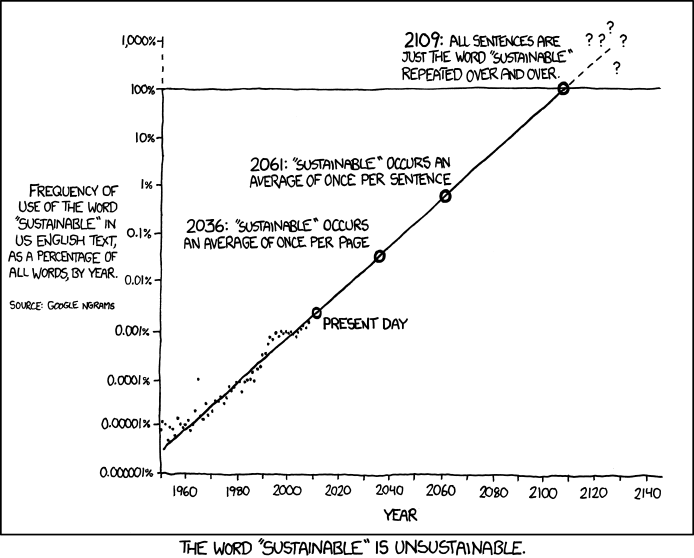
\includegraphics[width=2.5in]{extrap1.png}
\end{figure}
\vspace{-0.3cm}
Extrapolation brings trouble. It is important to ask the question for a new observation $\x^*$ if it is within the space of $\x$'s in the historical data. (Hardly anyone does this... but you should)! Be aware that extrapolation methods of different algorithms differ considerably! [R Demo]
	
\end{frame}

\begin{frame}\frametitle{Reconciliation of those Silly Cartoons}

\begin{figure}
\centering
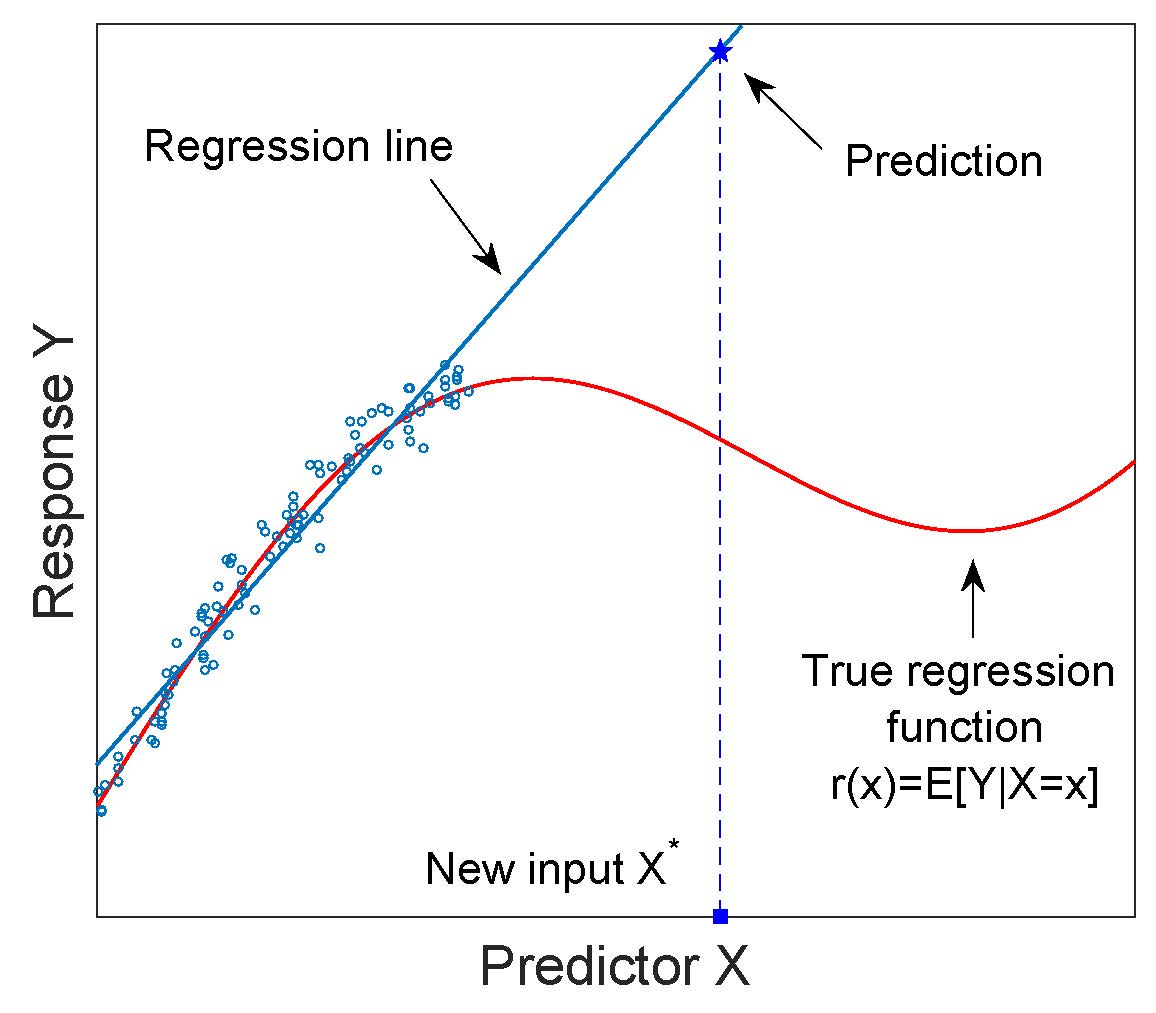
\includegraphics[width=3.2in]{extrap.jpg}
\end{figure}

\end{frame}

\begin{frame}\frametitle{Dataframe Design}

We spoke a lot about featurization i.e. selecting the columns in the dataframe (these are the predictors to measure). Once we did this, we can then go out and sample observations and then measure each for their predictor values. \\~\\ \pause

But we didn't speak at all about selecting the observations themselves (assuming you have some modicum of control of selecting your data). Two things to consider: \\~\\  \pause

\begin{enumerate}
\item \emph{Generalizability} refers to the ability of the model to generalize, or be \emph{externally valid} when considering new observations. This comes down to sampling observations from the same population as your new data you wish to predict (pretty obvious). Sometimes difficult in practice! \pause Extrapolation?? \pause
\item Optimal Design
\end{enumerate}

	
\end{frame}

\begin{frame}\frametitle{Optimal Design for Inferring one Slope}

Question: assume OLS and that we only care about inference for $\beta_1$. We can sample any $x$ values live in their set $\mathbb{X}$ e.g. $\in \bracks{x_m, x_M}$. What should the $n$ values be? \\~\\

Let $x_m = 0$, $x_M = 1$ and $n = 10$. The best inference for $\beta_1$ means ... \pause $\se{\betahat_1}$ is minimum. Design strategies for the $x$'s: \pause

\begin{enumerate}
\item Random sampling \pause
\item Uniform spacing: $\braces{0, 0.111, 0.222, \ldots, 0.999}$ \pause
\item Something else?
\end{enumerate}

[R demo]

\end{frame}


\begin{frame}\frametitle{Optimal Design: Split Between Extremes}

Recall the formula from Stat 102 / 613:

\beqn
\se{\betahat_1} = \sqrt{\frac{MSE}{(n-1)s^2_x}}
\eeqn

How can we make this small?

\begin{enumerate}
\item Maximize $n$ (duh)
\item Minimize the numerator, $MSE$ i.e. minimize the $SSE$. Can we do this? Yes by picking the closest $\betahat_1$ to $\beta_1$ (which we already do). \pause
\item Maximize the denominator $(n-1) s^2_x$. Since $n$ is already maximized, we can pick $x_1, \ldots, x_n$ to maximize $s^2_x$, the sample variance of the predictor.  How? \pause Put half of the $x$'s at $x_m$ and the other half at $x_M$ thereby \pause maximizing the distance from the $x$'s to \pause $\xbar$.
\end{enumerate}
	
\end{frame}

\begin{frame}\frametitle{Optimal Design of Linear Models}
\small

We seek the best linear approximation of $f(x)$ which is $\beta_0 + \beta_1 x _1+ \ldots + \beta_p x_p$. We pick the $\x$'s to give us the best linear approximation. What criteria? JMP gives two ways:

\begin{enumerate}
\item Note: $\var{\betahat_0, \betahat_1, \ldots, \betahat_p} = \sigsq \XtXinv$ \pause

$D$-optimality: maximize $\abss{\XtX}$ --- this maximizes the variance-covariance among the parameter estimates. \pause

\item Note: $\var{\Yhat_1, \ldots, \Yhat_n} = \sigsq \XXtXinvXt$ \pause

$I$-optimality: minimize the average prediction variance over the design space.
\end{enumerate}

[R Demo] \pause What did we learn? \pause For linear models with no polynomials or interactions, keep the observations as close to the minimimums and maximums as possible. For linear models with polynomials and interactions (more non-parametric than parametric), \pause keep most towards the minimums and maximums and some in the center of the input space.

\end{frame}



\section{Logistic Regression}


\begin{frame}\frametitle{Modeling Categorical Responses}

Previously the response $y$ was continuous and via the OLS assumptions we obtained the statistical model,

\beqn
Y \inddist \normnot{\beta_0 + \beta_1 x_1 + \ldots + \beta_p x_p}{\sigsq}
\eeqn

If the response $y$ is categorical, can we still use this? \pause No... the only elements in the support of the r.v. $Y$ are the levels only. [JMP Churn] \\~\\

First, assume $Y$ is binary i.e. zero or one. The model (AKA \qu{classifier}) we use is...\pause  

\beqn
Y \sim \bernoulli{f(x_1, \ldots, x_p)}
\eeqn

since $\cexpe{Y}{x_1, \ldots, x_p} = f(x_1, \ldots, x_p)$, then $f$ is still the conditional expectation function like before except now it varies only within \pause $\zeroonecl$ and it is the same as \pause   $\cprob{Y = 1}{x_1, \ldots, x_p}$.

\end{frame}

\begin{frame}\frametitle{Linear $f(x)$?}

We can model $f(x)$ as the simple linear function but this returns values smaller than 0 and larger than 1 and thus it cannot be the conditional expectation function! Why? \pause Lines vary between $\parens{-\infty, +\infty}$. \\~\\ \pause

We need a \qu{link function} to connect the linear function to the restricted support of the response:

\beqn
\lambda(f_{\reals}(x_1, \ldots, x_p)) = f(x_1, \ldots, x_p)
\eeqn

And the parametric assumption would be

\beqn
\lambda(s_{\reals}(x_1, \ldots, x_p; \theta_1, \ldots, \theta_\ell)) = s(x_1, \ldots, x_p; \theta_1, \ldots, \theta_\ell)
\eeqn

And assuming a linear form of $s_{\reals}$,

\beqn
\lambda(\beta_0 + \beta_1 x_1 + \ldots + \beta_p x_p) = ?
\eeqn

\end{frame}

\begin{frame}\frametitle{Choice of $\lambda$?}

We just need $\lambda: \reals \rightarrow \zeroonecl$. There are infinite $\lambda$'s to choose from. I've only seen three used: \pause

\begin{enumerate}
\item Logistic link: $\lambda(w) = \frac{e^w}{1 + e^w}$ (most common) \pause
\item Inverse normal (probit) link: $\lambda(w) = \Phi^{-1}(w)$ where $\Phi$ is the normal CDF function (somewhat common) \pause
\item Complementary Log-log (cloglog) link: $\lambda(w) = \natlog{-\natlog{w}}$ (rare!)
\end{enumerate}

Let's investigate what the first one means. Define $p := \prob{Y=1}$. We can think about probability  in another way:

\beqn
odds(Y = 1) := \frac{p}{1-p}
\eeqn

So if odds = 4:1, what is $p$? This means that the probability of the event happening is four times more likely than the complement happening. Or...  of 4+1 runs, 4 will be a yes. What is the range of odds? \pause $[0, \infty)$.
	
\end{frame}

\begin{frame}\frametitle{Why Logistic Link is Interpretable}
\small
Now let's take the log odds (called the logit function):

\beqn
logit(Y = 1) := \natlog{odds(Y = 1)} = \natlog{\frac{p}{1-p}}
\eeqn

What is the range of the logit function? \pause All of $\reals$. Hence, we can now set this equal to our \pause $s_\reals$ function. In the linear modeling context,

\footnotesize
\beqn
\beta_0 + \beta_1 x_1 + \ldots + \beta_p x_p &=& logit(Y = 1) =  \natlog{\frac{p}{1-p}} \\ \pause
e^{\beta_0 + \beta_1 x_1 + \ldots + \beta_p x_p} &=& \frac{p}{1-p} \\ \pause
(1-p)e^{\beta_0 + \beta_1 x_1 + \ldots + \beta_p x_p} &=& p \\ \pause
e^{\beta_0 + \beta_1 x_1 + \ldots + \beta_p x_p}  &=& p + p e^{\beta_0 + \beta_1 x_1 + \ldots + \beta_p x_p}\\ \pause
p &=& \frac{e^{\beta_0 + \beta_1 x_1 + \ldots + \beta_p x_p}}{1 + e^{\beta_0 + \beta_1 x_1 + \ldots + \beta_p x_p}} = \lambda(\beta_0 + \beta_1 x_1 + \ldots + \beta_p x_p) \pause
\eeqn

\small
Thus, a change in the linear model becomes a linear change in log-odds. This is (I would say) the most interpretable link function situation we've got.
	
\end{frame}

\begin{frame}\frametitle{The Logistic Function}

\begin{figure}
\centering
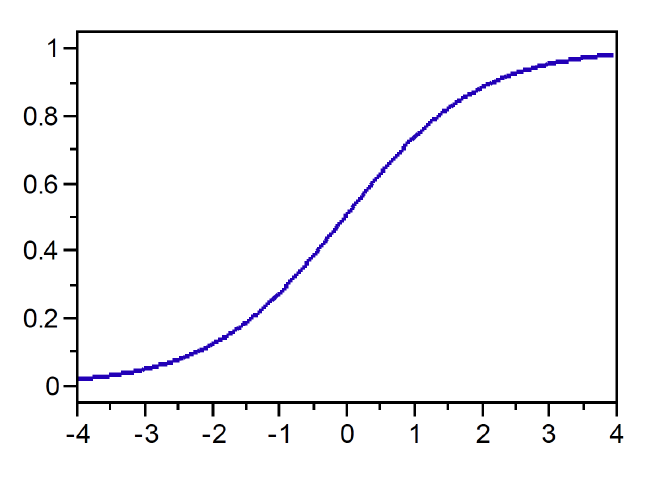
\includegraphics[width=3.2in]{logistic_function.png}
\end{figure}

\end{frame}

\begin{frame}\frametitle{How to Obtain a Model Fit}

A model fit would mean we estimate $\braces{\betahat_0, \betahat_1,  \ldots, \betahat_p}$. We initially did this estimation for regression (continuous $y$) by defining a loss function, SSE, and finding the optimal solution via calculus. What do we do now?? \\~\\

Likelihood to the rescue. First the \qu{logistic regression assumptions}

\begin{enumerate}
\item Linear-Logistic conditional expectation \pause
\item Independence
\end{enumerate}

\small
\beqn
&&\cprob{Y_1 = y_1, Y_2 = y_2, \ldots, Y_n = y_n}{\X_1 = \x_1, \X_2 = \x_2, \ldots, \X_n = \x_n} \\
&=& \prod_{i=1}^n \cprob{Y_i = y_i}{\X_1 = \x_i}
\eeqn

How?
	
\end{frame}

\begin{frame}\frametitle{Maximum Likelihood Estimates}
\small
\beqn
= \prod_{i=1}^n p^{y_i} (1-p)^{1-y_i}
\eeqn

How? \pause

\beqn
&& \lik{\beta_0, \beta_1, \ldots, \beta_p; \x_1, \ldots, \x_n} \\
&=& \prod_{i=1}^n \parens{\frac{e^{\beta_0 + \beta_1 x_1 + \ldots + \beta_p x_p}}{1 + e^{\beta_0 + \beta_1 x_1 + \ldots + \beta_p x_p}}}^{y_i} \parens{1 - \frac{e^{\beta_0 + \beta_1 x_1 + \ldots + \beta_p x_p}}{1 + e^{\beta_0 + \beta_1 x_1 + \ldots + \beta_p x_p}}}^{1-y_i}
\eeqn

How? \pause This does not have a simple, closed form solution. The computer iterates numerically using gradient methods. It usually uses the $\natlog{\cdot}$ of above, since it's (1) numerically more stable and (2) the expression is easier to work with. When it \qu{converges} on the values of the parameters that maximize the above, these are shipped to you as $\braces{\betahat_0, \betahat_1,  \ldots, \betahat_p}$. This is called \qu{running a logistic regression}. This usually is instant on a modern computer.
	
\end{frame}

\begin{frame}\frametitle{Prediction with Logistic Regression}
\small

How? \pause

\beqn
\phat = \phat(x^*_1, \ldots, x^*_p) = \pause \frac{e^{\betahat_0 + \betahat_1 x_1 + \ldots + \betahat_p x_p}}{1 + e^{\betahat_0 + \betahat_1 x_1 + \ldots + \betahat_p x_p}}
\eeqn
	
Note the predictions are for the conditional expectation function, the probability itself, the \emph{estimated expected probability}. However, you may actually wish to predict the response, the 1 or the 0. What to do?\\~\\ \pause

You can create a \emph{classification rule} which allows you to make a decision about the response based on the probability. What is the most intuitive classification rule? \pause

\beqn
\yhat = \indic{\phat \geq 0.5} := \pause \begin{cases} 1 ~~~\text{if}~~~ \phat \geq 0.5 \\ 0 ~~~\text{if}~~~ \phat < 0.5 \end{cases}
\eeqn

AKA the \qu{most likely criterion}. \pause We will return to prediction and evaluation of predictive performance later but first... inference.

\end{frame}


\begin{frame}\frametitle{Global Test in Logistic Regression}

\footnotesize
Recall in OLS regression, gaussian (normal) theory directly gave us $t$-tests and $F$-tests. Under the logistic regression assumptions, \emph{we have no such analogous theory}! However, we can make use of the ... \pause likelihood ratio test. Recall:

\vspace{-0.2cm}
\beqn
LR :=
%
\displaystyle \max_{\theta \in \Theta} \lik{\theta; x}
%
/
%
\displaystyle \max_{\theta \in \Theta_R}  \lik{\theta; x}
%
\eeqn

Let's now do a \qu{whole model} / \qu{global} / \qu{omnibus} test: \pause

\beqn
&& H_0: \beta_1 = 0, \beta_2 = 0, \ldots, \beta_p = 0, \quad H_a: \text{at least one is non-zero}
\eeqn

So $\Theta$ would be the space of all $\beta_0, \beta_1, \ldots, \beta_p$ and $\Theta_R$ will restrict the space to only $\beta_0$ with zeroes for all other \qu{slope} parameters.

\beqn
LR &=& \frac{
\displaystyle \max_{\beta_0, \beta_1, \ldots, \beta_p} 
\lik{\beta_0, \beta_1, \ldots, \beta_p; y_1, \ldots, y_n, \x_1, \ldots, \x_n}
}{
\displaystyle \max_{\beta_0} 
\lik{\beta_0, \beta_1 = 0, \ldots, \beta_p = 0; y_1, \ldots, y_n, \x_1, \ldots, \x_n}
}
\eeqn \pause


So on top the computer iterates to find $\braces{\betahat_0, \betahat_1,  \ldots, \betahat_p}$, plugs it in and computes the likelihood and on the bottom the computer independently iterates to find $\braces{\betahat_0}$, plugs it in and computes the likelihood, then together, the $LR$.
\end{frame}

\begin{frame}\frametitle{Partial Tests in Logistic Regression}

\small
We then look at $Q = 2\natlog{LR}$ and compare it to the appropriate $\chi^2$ distribution. Here, since we've dropped $p$ parameters / degrees of freedom, we look at the critical $\chisq{p, \alpha}$ value.\\~\\ \pause

Let's say we want to test something like:

\beqn
&& H_0: \beta_1 = 0 ~\&~ \beta_2 = 0, \quad H_a: \text{at least one is non-zero}
\eeqn

We can again use the likelihood ratio test:

\beqn
LR = \frac{
\displaystyle \max_{\beta_0, \beta_1, \ldots, \beta_p} 
\lik{\beta_0, \beta_1, \ldots, \beta_p; y_1, \ldots, y_n, \x_1, \ldots, \x_n}
}{
\displaystyle \max_{\beta_0, \beta_3, \ldots, \beta_p} 
\lik{\beta_0, \beta_1 = 0, \beta_2 = 0, \beta_3, \ldots, \beta_p = 0; y_1, \ldots, y_n, \x_1, \ldots, \x_n}
}
\eeqn \pause

We then look at $Q = 2\natlog{LR}$ and compare it to the appropriate $\chi^2$ distribution. Here, since we've dropped $2$ parameters / degrees of freedom, we look at the critical $\chisq{2, \alpha}$ value.\\~\\ \pause

\end{frame}

\begin{frame}\frametitle{Individual Tests in Logistic Regression}

Let's say we want to test an individual slope coefficient:

\beqn
&& H_0: \beta_j = 0, \quad H_a: \beta_j \neq 0
\eeqn
	
We can again use the likelihood ratio test:

\footnotesize
\beqn
\hspace{-10pt} LR = \frac{
\displaystyle \max_{\beta_0, \beta_1, \ldots, \beta_p} 
\lik{\beta_0, \beta_1, \ldots, \beta_p; y_1, \ldots, y_n, \x_1, \ldots, \x_n}
}{
\displaystyle \max_{\beta_0, \beta_1, \ldots, \beta_{j-1}, \beta_{j+1}, \ldots \beta_p} 
\lik{\beta_0, \beta_1, \ldots, \beta_{j-1}, \beta_j = 0, \beta_{j+1}, \ldots \beta_p; y_1, \ldots, y_n, \x_1, \ldots, \x_n}
}
\eeqn \pause

\small
We then look at $Q = 2\natlog{LR}$ and compare it to the appropriate $\chi^2$ distribution. Here, since we've dropped 1 parameter / degrees of freedom; thus we look at the critical $\chisq{1, \alpha}$ value. \\~\\ \pause

There is something special about a $\chisq{}$ r.v. with one degree of freedom. \pause Note this cool fact from probability theory: $\sqrt{\chisq{1}} \sim \stdnormnot$ i.e. a \qu{z-score}. This is how JMP produces standard errors for logistic regression coefficients.

\end{frame}


\begin{frame}\frametitle{Telecom Company Churn Example}
\small
In marketing \qu{churn} refers to a customer canceling their service. Studies suggest that it costs 5-10x more to acquire a new customer than to retain an old customer. Thus, predicting churn is of major interest! \\~\\ \pause

Here's a dataset from a telecom company (likely it's churn on Verizon / AT\&T / T-Mobile /Sprint's cell-phone plan). We have 7,043 customers with 20 features. This is likely a nearly-mindless dump!! Churn is defined to be a complete cancellation of services in the next month period. Since we are predicting churn, define $y=1$ to be churn, so the $\phat$'s are estimates of probability of churning (this just makes everything easier to understand). \\~\\ \pause

We begin just trying to model $y$: churn vs. $x$: tenure (the number of months customer is currently subscribed for). What do you think the relationship will be? $\partial /\partial x [f(x)]$?
	
\end{frame}

\begin{frame}\frametitle{Results of Simple Logistic Regression}

[JMP demo] Which likelihood numbers are best? Well highest likelihoods are good which means highest log likelihoods which means \textit{smallest} negative log likelihoods.... yup it's confusing. Here's what JMP did:

\beqn
Q &=& 2\natlog{LR} = 2\parens{\loglik{\thetahat; x} - \loglik{\thetahat_R; x}} \\
&=& 2\parens{-(3595.9341) - -(4075.0729)}\\
&=& 2\parens{479.1389} = 958.2778  \\
&=& 2\natlog{1.22 \times 10^{208}}
\eeqn

and $\chisq{1, 5\%}$ = \texttt{qchisq(.95, 1)} = 3.84. So this passes the test (comfortably). We reject $H_0$ and conclude that the model is linearly useful. \pause ALSO: equivalent to a test of one variable. We reject $H_0$ and conclude tenure has a linear effect on the log-odds of churn. \\~\\ \pause

	
\end{frame}

\begin{frame}\frametitle{Basic Predictions I}

Predict estimated expected probability of churn for someone who has 1 month of tenure

\beqn
\phat = \frac{e^{\betahat_0 + \betahat_1 x_1}}{1 + e^{\betahat_0 + \betahat_1 x_1}} = \frac{e^{0.0273 + (-0.0288) (1)}}{1 + e^{0.0273 + (-0.0288) (1)}} = \frac{0.9985}{1.9985} = 0.500
\eeqn

How about 2 months of tenure?

\beqn
\phat = \frac{e^{\betahat_0 + \betahat_1 x_1}}{1 + e^{\betahat_0 + \betahat_1 x_1}} = \frac{e^{0.0273 + (-0.0288) (2)}}{1 + e^{0.0273 + (-0.0288) (2)}} = \frac{0.9702}{1.9702} = 0.492
\eeqn

i.e. a difference in about 0.8\% as measured on a probability scale.

\end{frame}

\begin{frame}\frametitle{The Logistic Function}

\begin{figure}
\centering
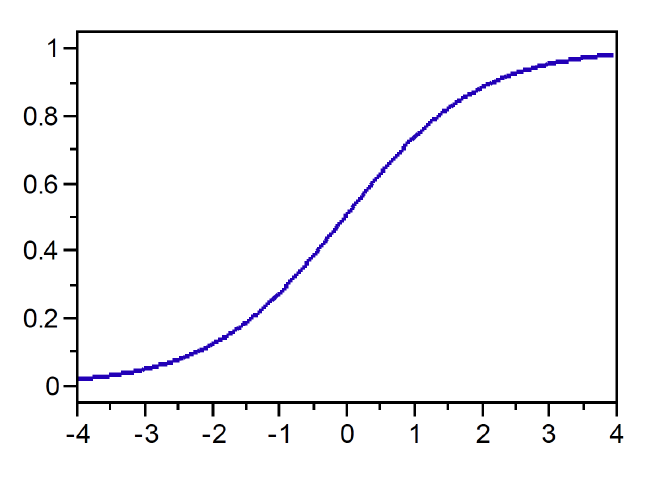
\includegraphics[width=3.2in]{logistic_function.png}
\end{figure}

A move of one unit in $x$ when $x \approx 0$ is a much bigger move than one unit in $x$ when $x \approx 3$

\end{frame}

\begin{frame}\frametitle{Parameter Standard Error}

To add to the confusion... JMP prefers to calculate parameter estimates and standard error via the Wald test, which is similar to the likelihood ratio test. Thus, 761.00 $\neq$ 958.28 but, remarkably, they are about the same conceptually -- both large and significant. The standard errors,

\beqn
\underbrace{Q = z^2}_{\substack{\text{fact from} \\ \text{probability} \\ \text{theory}}} = \squared{\frac{\betahat_1}{s_{\betahat_1}}} \Rightarrow  s_{\betahat_1} = \frac{\abss{\betahat_1}}{\sqrt{Q}}
\eeqn

are expectedly about the same 

\beqn
s_{\betahat_1} &=& \frac{\abss{-0.0387682}}{\sqrt{761.00}} = 0.0014 \eqncomment{via the Wald test}\\
s_{\betahat_1} &=& \frac{\abss{-0.0387682}}{\sqrt{958.28}} = 0.0013 \eqncomment{via the LR test}
\eeqn

	
\end{frame}



\begin{frame}\frametitle{Multivariate Logistic Regr. Interp. I}

Now let's use all variables. Questions:

\begin{itemize}
\item Which variable(s) should we leave out? \pause \texttt{customerID} --- no causal mechanism.
\item Why are we getting biased estimates and zeroes? \pause Perfect multicollinearity. \pause  Solution? \pause Kill columns until you don't get the error anymore. Turns out 6 have to be removed.
\end{itemize}

\end{frame}

\begin{frame}\frametitle{Realistic Predictors Illustration (updated)}

\begin{figure}
\centering
\hspace{-0.5cm}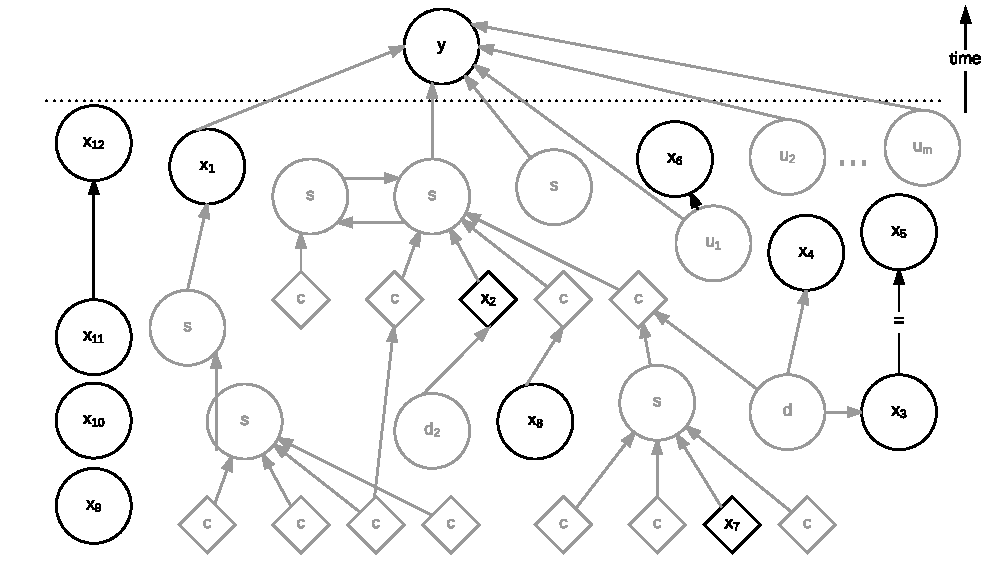
\includegraphics[width=4.6in]{realistic_predictors}
\end{figure}
	
\end{frame}

\begin{frame}\frametitle{Multivariate Logistic Regr. Interp. II}

\small
Now let's use all variables. Questions:

\begin{itemize}
\item \ingrey{Which variable(s) should we leave out? \texttt{customerID} --- no causal mechanism.}
\item \ingrey{Why are we getting biased estimates and zeroes?  Perfect multicollinearity.}
\item Are all these variables \qu{significant}? \pause No. After a Bonferroni correction, we \qu{lose} two. Are they for sure insignificant? \pause No, maybe we didn't have enough power to detect them...
\item Do the coefficients sign / size make sense intuitively? \pause Yes?
\item Which of the \qu{driving} variables are \textit{not} able to be manipulated? \pause Senior citzen, total charges (?) \pause
\item Should you (the manager) try to incentivize electronic checks? \pause Paperless billing? \pause Dropping multiple phone lines? \pause You can try these things if you have nothing to lose, but remember, they are not guaranteed to be causal! And they may \inred{backfire!!} (Can you think of an example??)
\end{itemize}

\end{frame}

\begin{frame}\frametitle{Remember Where you At!!}

\begin{figure}
\centering
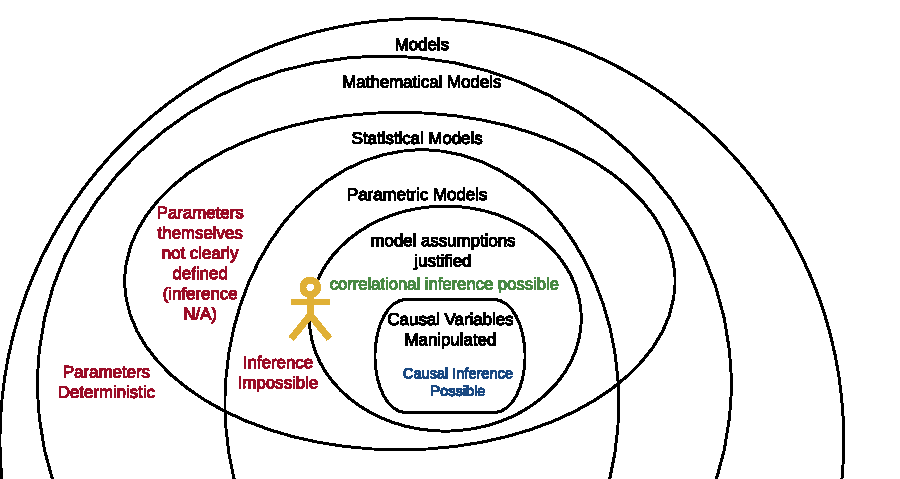
\includegraphics[width=4.75in]{where_we_at}
\end{figure}

	
\end{frame}

\begin{frame}\frametitle{Evaluating Logistic Regression Models}

Many, many measures reported by JMP that we generally don't use: \pause

\begin{itemize}
\item $R^2(U)$
\item Generalized $R^2$
\item Mean Negative Log probability
\item \qu{RMSE}
\item Mean Absolute Deviation \pause
\end{itemize}

And ones that we do use:

\begin{itemize}
\item AICc / BIC (for something a little bit different... we will come back to this in a couple of lectures) \pause
\item Misclassification Rate \pause
\end{itemize}

We now cover evaluating classification models in general (not only in the context of logistic regression models specifically).

\end{frame}

\section{Evaluating Classification Models}

\begin{frame}\frametitle{Probability Predictions $\Rightarrow$ Level Predictions}

\small
Recall that ... you can create a classification rule which allows you to make a decision about the response based on the probability. The most intuitive classification rule is: \pause

\beqn
\yhat = \indic{\phat \geq 0.5} := \pause \begin{cases} 1 ~~~\text{if}~~~ \phat \geq 0.5 \\ 0 ~~~\text{if}~~~ \phat < 0.5 \end{cases}
\eeqn

In regression, you examined functions of the residuals $e_i := y_i - \yhat_i$ to assess model fit. What is an analagous residual here? There are four residuals, two representing errors. The best way to see them is to create the \emph{confusion matrix}:

\begin{table}
\centering
\begin{tabular}{cc|cc|}
& & \multicolumn{2}{c|}{$\yhat$ (decision)} \\
& & 1 & 0 \\ \hline
\multirow{2}{*}{$y$ (truth)} & 1 & true positive (TP) & false negative (FN) \\ 
& 0 & false positive (FP) & true negative (TN) \\ \hline
\end{tabular}
\end{table}

Why do \qu{correlations rock} here?? \pause We are purely evaluating predictive performance... no inferential claims!

\end{frame}


\begin{frame}\frametitle{Confusion Matrix for Churn Model}

JMP gives us the matrix [JMP], \pause but they don't annotate it well. Here are some numbers I like to see:

\footnotesize
\begin{table}
\centering
\begin{tabular}{cc|cc|cc}
& & \multicolumn{2}{c|}{$\yhat$} & & Model \\
& & 1 & 0 & Totals &  Errors\\ \hline
\multirow{2}{*}{$y$} & 1 & $TP$ = 1012 & $FN$ = 857 & $P$ = 1869 & $FNR$ = 45.9\% \\ 
& 0 & $FP$ = 531 & $TN$ = 4632 & $N$ = 5163 & $FPR$ = 10.2\% \\ \hline
& Totals & $\Phat$ = 1543 & $\Nhat$ = 5489 & $n=$ 7032 \\
& Use errors & $FDR$ = 34.3\% & $FOR$ = 15.6\% & & \fbox{$ME$ = 19.7\%}
\end{tabular}
\end{table}
\normalsize

There are other metrics commonly reported


\begin{itemize}
\item Sensitivity = Recall = $\frac{TP}{TP + FN} = \frac{TP}{P}$, the proportion of positives successfully recovered (large value = good model), 54.9\% above
\item Specificity = $\frac{TN}{TN + FP} = \frac{TN}{N}$, the proportion of negatives successfully recovered (large value = good model), 89.8\% above
\end{itemize}
	
\end{frame}


\begin{frame}\frametitle{Misclassification Error}

Already... what is one broad, general metric to evaluate the model? Misclassification error cost function (or Accuracy):

\beqn
ME &:=& \oneover{n} \sum_{i=1}^n \indic{y_i \neq \yhat_i} \\
ACC &:=& 1 - ME = \oneover{n} \sum_{i=1}^n \indic{y_i = \yhat_i}
\eeqn

This essentially treats both types of errors (FN and FP) equally (more on this later).
	
\end{frame}

\begin{frame}\frametitle{Production Classifier Flowchart}
\begin{figure}
\centering
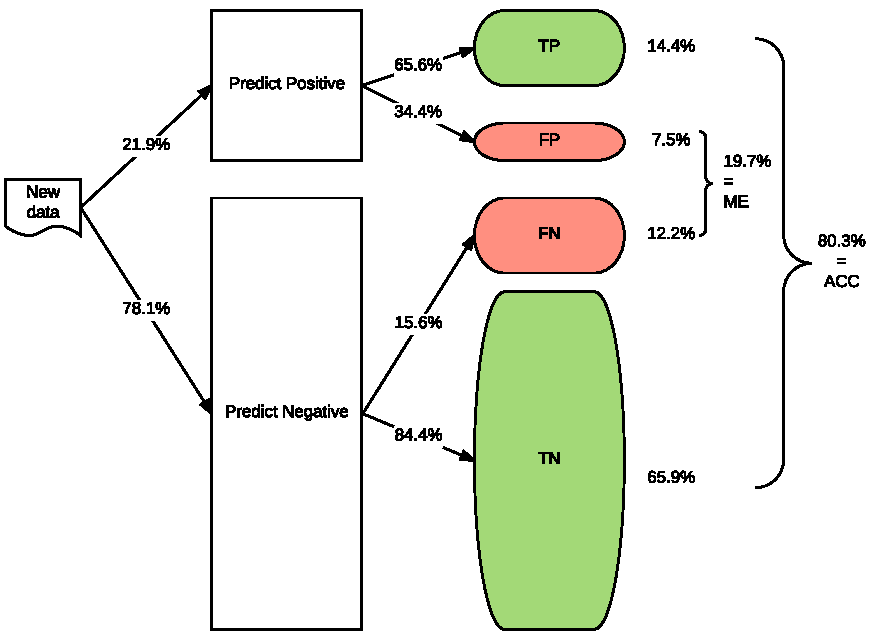
\includegraphics[width=3.95in]{classifier_flowchart}
\end{figure}
\end{frame}


\begin{frame}\frametitle{There's a Ton of Metrics...}

From \href{https://en.wikipedia.org/wiki/Confusion\_matrix\#Table\_of\_confusion}{wikipedia}... 

\begin{figure}
\centering
\hspace{-0.5cm}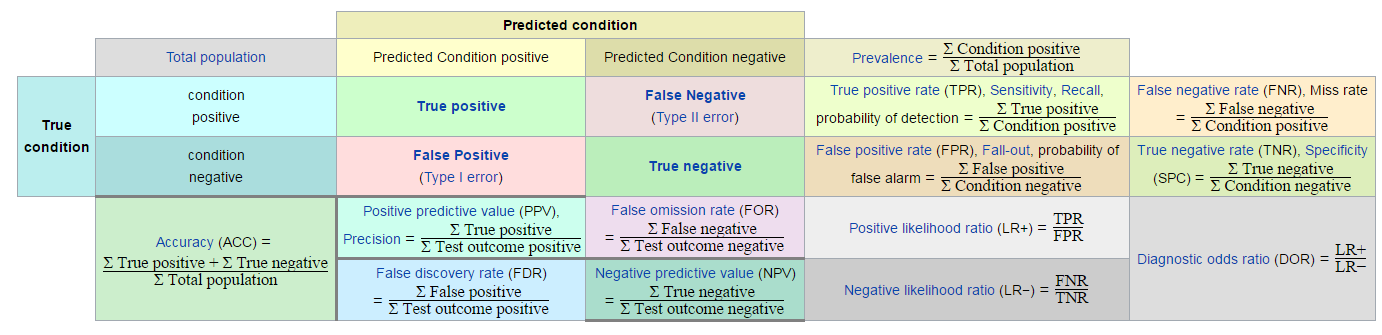
\includegraphics[width=4.25in]{confusion_matrix.png}
\end{figure}

\footnotesize
Others (from above) commonly used:

\begin{itemize} \footnotesize
\item False Discovery Rate (FDR) = $\frac{FP}{TP + FP} = \frac{FP}{\Phat}$, the proportion of negatives of those predicted to be positive (small value = good model) \pause
\item False Omission Rate (FOR) = $\frac{FN}{TN + FN} = \frac{FN}{\Nhat}$, the proportion of postives of those predicted to be negative (small value = good model) \pause
\item Precision = Positive Predictive Value (PPV) = 1 - FDR = $\frac{TP}{TP + FP}$, the proportion of postives of those predicted to be positive (large value = good model)
\end{itemize}
	
\end{frame}


\begin{frame}\frametitle{One Way to Think About Classification}


\end{frame}



\begin{frame}\frametitle{Generalizing the Classification Rule}

Recall the classification rule $\yhat = \indic{\phat \geq 0.5}$. Using 0.5 is a principled default but we can use any rule $p_0 \in (0,1)$:

\beqn
\yhat = \indic{\phat \geq p_0} := \pause \begin{cases} 1 ~~~\text{if}~~~ \phat \geq p_0 \\ 0 ~~~\text{if}~~~ \phat < p_0 \end{cases}
\eeqn

What happens when we change the $p_0$ threshold? If $p_0 \uparrow ~~\Rightarrow~~ \Phat \pause \downarrow$ and $\Nhat \pause \uparrow$. If $p_0 \downarrow ~~\Rightarrow~~ \Phat \pause \uparrow$ and $\Nhat \pause \downarrow$. Changing $p_0$ changes the column totals and obviously creates a whole new confusion matrix.
\\~\\

So now it's simple, vary $p_0$ and pick the best model according to your cost / error / loss function (the $ME$ at the moment). Let's just do every $p_0$!
	
\end{frame}

\begin{frame}\frametitle{Receiver-Operator Characteristic Table}

\begin{figure}
\centering
\hspace{-0.5cm}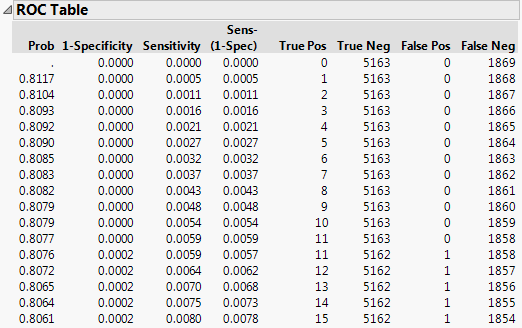
\includegraphics[width=3.0in]{roc_table.png}
\end{figure}

\vspace{-0.3cm}
Here, \texttt{Prob} is what we denoted $p_0$. \qu{Best model} is not defined here by highest $ACC$ (lowest $ME$), it's determined by highest \textbf{specificity + sensitivity} or equivalently, the highest \textbf{sensitivity - (1 - specificity)}.JMP indicates that row with a $\star$. This is an arbitrary metric, but is a good default.

\end{frame}

\begin{frame}\frametitle{Receiver-Operator Characteristic Curve}

\vspace{-0.2cm}
\begin{figure}
\centering
\hspace{-0.5cm}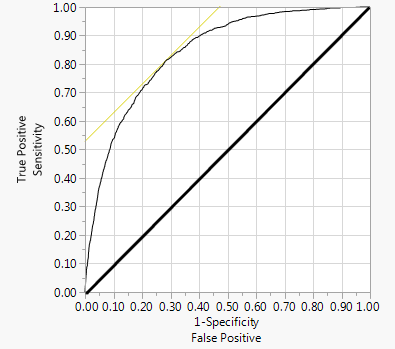
\includegraphics[width=2.4in]{roc_curve.png}
\end{figure}

\small
\vspace{-0.3cm}
This is graphical illustration of the table. Each dot represents the sensitivity-specificity tradeoff for each $p_0$. \pause The starred row of maximum sensitivity + specificity is indicated here by a yellow tangent line. \pause I drew the diagonal line to indicate predictive performance that is expected \qu{by chance}. Why? \pause Also, are there other ROC variants? \pause Yes.

\end{frame}


\begin{frame}\frametitle{Area Under the Curve (AUC) Metric}

\vspace{-0.2cm}
\begin{figure}
\centering
\hspace{-0.5cm}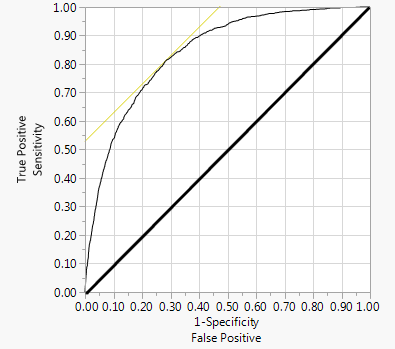
\includegraphics[width=1.3in]{roc_curve.png}
\end{figure}

\small
\vspace{-0.3cm}
If you built a model by chance the \qu{area under the curve} (or to the right of the curve) on the graph would be ... \pause 0.5 since the graph is a unit square. Under the ROC curve itself (or to its right) is an area ... \pause greater than 0.5. Here, it's 0.844. \pause This metric is called AUC and is widely used as a metric to assess performance of all possible classifiers in this set of models together, it is a composite metric unlike $ME$ or anything derived from an individual confusion table.\\~\\

AUC is nice to evaluate overall performance of all possible models... but at the end of the day... \pause you ship \emph{ONE} model! So we still need a means of evaluating our one model from one confusion table.

\end{frame}


\begin{frame}\frametitle{Churn Example Where $p_0 = 0.10$}
\pause
\tiny
\begin{table}
\centering
\begin{tabular}{cc|cc|cc}
& $p_0 = 0.5$ & \multicolumn{2}{c|}{$\yhat$} & & Model \\
& & 1 & 0 & Totals &  Errors\\ \hline
\multirow{2}{*}{$y$} & 1 & $TP$ = 1012 & $FN$ = 857 & $P$ = 1869 & $FNR$ = 45.9\% \\ 
& 0 & $FP$ = 531 & $TN$ = 4632 & $N$ = 5163 & $FPR$ = 10.2\% \\ \hline
& Totals & $\Phat$ = 1543 & $\Nhat$ = 5489 & $n=$ 7032 \\
& Use errors & $FDR$ = 34.3\% & $FOR$ = 15.6\% & & \fbox{$ME$ = 19.7\%}
\end{tabular}
\end{table}
\normalsize
\pause

\footnotesize
\begin{table}
\centering
\begin{tabular}{cc|cc|cc}
& $p_0 = 0.1$ & \multicolumn{2}{c|}{$\yhat$} & & Model \\
& & 1 & 0 & Totals &  Errors\\ \hline
\multirow{2}{*}{$y$} & 1 & $TP$ = 1772 & $FN$ = 97 & $P$ = 1869 & $FNR$ = 5.1\% \\ 
& 0 & FP = 2669 & $TN$ = 2494 & $N$ = 5163 & $FPR$ = 51.6\% \\ \hline
& Totals & $\Phat$ = 4441 & $\Nhat$ = 2591 & $n=$ 7032 \\
& Use errors & $FDR$ = 60.1\% & $FOR$ =3.7\% & & \fbox{$ME$ = 39.3\%}
\end{tabular}
\end{table}\pause
\small


Which numbers did not change? \pause $n$, $P$ and $N$. Why? \pause These are fixed according to the dataframe. All other numbers changed! What happend to our first means of evaluation, the Misclassification Error? \pause It increased from 19.7\% $\rightarrow$ 39.3\%. So isn't this a worse model?? \\~\\ \pause 

Not necessarily... It depends on what your goal is!
\end{frame}

\begin{frame}\frametitle{Asymmetric Costs in a Classifier}

These are always two types of errors but the costs are not always the same.

\tiny
\begin{table}
\centering
\begin{tabular}{cc|cc|cc}
& $p_0 = 0.1$ & \multicolumn{2}{c|}{$\yhat$} & & Model \\
& & 1 & 0 & Totals &  Errors\\ \hline
\multirow{2}{*}{$y$} & 1 & $TP$ = 1772 & $FN$ = 97 & $P$ = 1869 & $FNR$ = 5.1\% \\ 
& 0 & FP = 2669 & $TN$ = 2494 & $N$ = 5163 & $FPR$ = 51.6\% \\ \hline
& Totals & $\Phat$ = 4441 & $\Nhat$ = 2591 & $n=$ 7032 \\
& Use errors & $FDR$ = 60.1\% & $FOR$ = 3.7\% & & \fbox{$ME$ = 39.3\%}
\end{tabular}
\end{table}\pause
\small

Imagine we really are the Telecom business manager. It costs 5-10x more to acquire a new customer than to engage a customer who is likely to churn. What type of error specifically is \textit{very} costly? \pause The $FN$. Who are they? \pause These are those who you said were not going to churn \textit{and they did}! Cost? \pause You need to acquire a new customer! The other type of error is less costly, the $FP$. Who are they? \pause These are the people you thought were going to churn and did not. Cost? \pause Whatever the incentive package is.
	
\end{frame}

\begin{frame}\frametitle{Weighted Misclassification Error}

We now define two costs: (1) the cost of the $FP$ denoted $c_{FP}$ and (2) the cost of the $FN$ denoted $c_{FN}$. We then define the weighted misclassification error evaluation metric:

\beqn
ME_w := \oneover{n} \sum_{i=1}^n c_{FP} \indic{y_i = 0 \& \yhat = 1} + c_{FN} \indic{y_i = 1 \& \yhat_i = 0}
\eeqn

We now vary $p_0$ to locate the model that optimizes this error to be minimum.
	
\end{frame}

\begin{frame}\frametitle{Minimum Weighted Misclassification Error}

Let's assume that $c_{FN} = \$1000$ and $c_{FP} = \$100$ just for the example's sake. Note: this is a \emph{cost ratio} of 10:1.

\vspace{-0.2cm}
\begin{figure}
\centering
\hspace{-0.5cm}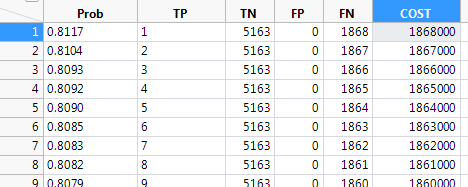
\includegraphics[width=3.1in]{weighted_misclassification_costs.png}
\end{figure}

We now calculate the cost and find the minimum model (i.e. the $p_0$ to ship). [JMP] \pause Or alternatively, we can select the model with the closest $FN / FP \approx 10:1$ to match the stakeholder preference of the desired cost ratio.



	
\end{frame}

\begin{frame}\frametitle{Expected Value Calculation}

You can also imagine assignment of both costs \textit{and} benefits:

\tiny
\begin{table}
\centering
\begin{tabular}{cc|cc|}
& $p_0 = 0.1$ & \multicolumn{2}{c|}{$\yhat$}   \\
& & 1 & 0  \\ \hline
\multirow{2}{*}{$y$} & 1 & $b_{TP}$ & $c_{FN}$  \\ 
& 0 & $c_{FP}$ &$b_{TN}$  \\ \hline
\end{tabular}
\end{table}\pause
\small

and then use the confusion matrix to estimate probabilities:

\begin{table} \small
\centering
\begin{tabular}{cc|cc|}
& $p_0 = 0.1$ & \multicolumn{2}{c|}{$\yhat$}  \\
& & 1 & 0 \\ \hline
\multirow{2}{*}{$y$} & 1 & 25.1\% & 1.3\%  \\ 
& 0 & 40.0\% & 35.5\%  \\ \hline
\end{tabular}
\end{table}\pause
\small

The expected value would be? 

\beqn
\expe{T} &=& p_{TP} \times b_{TP} +  p_{TN} \times b_{TN} + p_{FP} \times c_{FP} +  p_{FN} \times c_{FN} \\
&\approx& \phat_{TP} \times b_{TP} +  \phat_{TN} \times b_{TN} + \phat_{FP} \times c_{FP} +  \phat_{FN} \times c_{FN}
\eeqn

Highest expected value model is shipped (ex. from Provost \& Fawcett, 2013).
	
\end{frame}

\begin{frame}\frametitle{$\phat$'s as Ordinal Values}

One final point... If we were on a mission to find the top $m$ churners. What would we do? \pause Sort the $\phat$'s and return the top $m$.
	
\end{frame}


\end{document}
	


\begin{frame}\frametitle{}

	
\end{frame}

\begin{frame}\frametitle{}

	
\end{frame}

\begin{frame}\frametitle{}

	
\end{frame}






\begin{frame}\frametitle{}

	
\end{frame}



\begin{frame}\frametitle{}

	
\end{frame}

\begin{frame}\frametitle{}

	
\end{frame}


\begin{frame}\frametitle{}

	
\end{frame}

\begin{frame}\frametitle{}

	
\end{frame}


\begin{frame}\frametitle{}

	
\end{frame}

\begin{frame}\frametitle{}

	
\end{frame}


\begin{frame}\frametitle{}

	
\end{frame}

\begin{frame}\frametitle{}

	
\end{frame}


\begin{frame}\frametitle{}

	
\end{frame}

\begin{frame}\frametitle{}

	
\end{frame}


\begin{frame}\frametitle{}

	
\end{frame}

\begin{frame}\frametitle{}

	
\end{frame}


\begin{frame}\frametitle{}

	
\end{frame}

\begin{frame}\frametitle{}

	
\end{frame}


\begin{frame}\frametitle{}

	
\end{frame}

\begin{frame}\frametitle{}

	
\end{frame}


\begin{frame}\frametitle{}

	
\end{frame}

\begin{frame}\frametitle{}

	
\end{frame}